\spaltenanfang



\abschnitt{Überblick}
Im \textbf{Greifenfurt}er Umland erfahren die Helden von einem Ork-Überfall, bei dem der \textbf{Knappe Alfdan} entführt wurde, und nehmen die Verfolgung auf.
Die Fährte führt zu einer Klamm, wo sich die Orks eingenistet haben, um von hier aus \textbf{Gut Nebelstein} zu erobern.
Nur mit List und Geschick werden es die Helden schaffen, die Orks und ihre Handlanger zu überwinden, den \textbf{Knappen Alfdan} zu befreien und dem plötzlich auftauchenden Elitetrupp des Ork-Schamanen \textbf{Shurrak Windzahn} zu entkommen.
\info{
\textbf{Die Erfahrungsstufe der Helden}

Dieses Abenteuer ist für 2-4 \textit{unerfahrene Neulinge} (2000~EP) konzipiert. Falls sich die Abenteuergruppe noch nicht kennt, wird sie im Vorlesetext zusammengeführt.
}

\abschnitt{Der Weg ins Abenteuer}

\info{
\textbf{Vorlesetexte}

Den folgenden Text kannst du deiner Gruppe direkt vorlesen. Lies ihn dir im Vorfeld einmal in Ruhe durch. Trage ihn dann am Spieltisch mit lebhafter Stimme vor.
}

\vorlesen{Langsam sinkt die kalte Herbstsonne hinter das \textbf{Finsterkamm}-Gebirge und taucht das Tal um \textbf{Gut Nebelstein} in tiefe Schatten. 
	Es klang nach einem bedeutsamen Auftrag, als die alte Ritterin, \textbf{Wahntraude von Rebenich}, euch in ihre Dienste nahm:
	In die Stadt Greifenfurt solltet ihr reisen und dort der \textbf{Markgräfin} die Unterstützung anbieten, um die sie angesichts der großen Bedrohung aus dem Norden schon seit langer Zeit verzweifelt bat.
	\textbf{Wahntraude} hat daher eine Gruppe an Abenteurern auf den Weg geschickt. Ihr seid \dots}

\info{
Fordere die Personen am Spieltisch nun auf, ihre Helden mit Namen und Aussehen kurz vorzustellen!
}

\vorlesen{Ihr wart schon ein gutes Stück entlang des sich talwärts mäandernden Baches gewandert, da lief euch jedoch eine Dienerin in die Arme:
	\textbf{Treudane Degenhardt}, von Dornenbüschen zerkratzt und völlig außer Atem.
	Sie war gemeinsam mit \textbf{Alfdan}, dem Knappen von Gut Nebelstein, und dessen Mutter und Gärtnerin \textbf{Alwena} auf dem Rückweg vom Markt in Greifenberg gewesen.
	Ein Dutzend grobschlächtiger Orks hat sie überfallen, wenige Meilen von hier, und den jungen \textbf{Alfdan} samt Markterlös in die Berge gezerrt.
	
	Die fürsorgliche Ritterin wird völlig aufgelöst sein, wenn sie davon erfährt, dass ihr einziger Knappe ihren Feinden in die Hände fällt! Und das wird zweifellos geschehen, wenn ihr nichts unternehmt!}

\info{
\textbf{Gelenkte Passagen}

Wie du sicherlich bemerkt hast, haben die Helden hier nicht wirklich eine Wahl, was zu tun ist. Solche Passagen können sinnvoll sein, um das Abenteuer ohne große Umwege zu starten. Damit allen am Spieltisch sofort klar ist, dass hier keine Interaktionsmöglichkeiten bestehen, ist der Vorlesetext in der Vergangenheitsform geschrieben.
}

\vorlesen{Ihr wart also sofort zum Ort des Verbrechens geeilt, um die noch frische Fährte aufzunehmen und die Entführer einzuholen. Beim zurückgelassenen Ochsenkarren stockte euch der Atem:
	Zwischen zerschlagenen Weidenkörben und zerstreuten Äpfeln lag dort blutüberströmt eine Frau, deren noch zitternde Hand auf etwas in der Ferne zu deuten schien.
	Mit letzter Kraft hauchte sie euch entgegen: „Sie haben \dots\ mein Sohn \dots“
	Da nicht mehr aus ihr herauszubekommen war, als Boron sie zu sich nahm, folgten eure Blicke ihrer nun toten Hand:
	Sie zeigte auf die Hänge des \textbf{Finsterkamm}s.
	Sofort seid ihr losgeeilt und eine ab und an sichtbare Fährte aus Bluttropfen führte euch immer höher ins Gebirge.
	Schließlich endete die Spur in einem dunklen Höhleneingang.}
\spaltenende
\begin{center}
\zeichnung[0.6\textwidth]{pferd.jpg}
\end{center}
\newpage

\spaltenanfang
\abschnitt{Höhleneingang}
\vorlesen{Als ihr einen vorsichtigen Blick hineinwagt, schlägt euch Verwesungsgeruch entgegen.
	Im Dämmerlicht der von außen eindringenden Abendröte könnt ihr Tierknochen erkennen, die den ganzen Boden bedecken.
	Als ihr einen Moment den Atem anhaltet, hört ihr ein Nagen.
	
Was tut ihr?}


\info{
Jetzt erfährst du, was die Gruppe hier entdecken könnte!
}

In der Höhle liegt ein toter \textbf{Ork} (aschfarbene Haut, dichte schwarze Behaarung, breite Nase, dominanter Überaugenwulst, Unterbiss mit hervorstechenden Eckzähnen, spitze Ohren), den gerade ein Schwarm Ratten abnagt.

Er wurde kürzlich von einem Schwert in den Bauch gestoßen, hat sich noch in die Höhle geschleppt und ist dann umgefallen und verblutet.
Sein rechter Arm ragt in einen großen Haufen Unrat.

Wer seine Hand freilegt, sieht, dass sich, unter dem Haufen versteckt, eine aufschiebbare hölzerne Bodenabdeckung befindet, die der Tote offenbar öffnen wollte. Diese Abdeckung ist außerdem etwas zu kurz geraten und lässt nach vorne hin eine kleine Lücke.

Bei einer Bedrohung durch Feuer fliehen einige der Ratten in den darunter liegenden Abgang (\textbf{Mine}).

\abschnitt{Mine}
\vorlesen{Ihr steigt den Abgang in die Finsternis hinab. Fast schnurgerade führt der enge Stollen in den Berg hinein. Die Gesteinswände sind feucht und glitschig. Ab und zu fällt ein dicker Wassertropfen auf euren Kopf.
	Die niedrige, tief zerfurchte Decke ist alle paar Schritt notdürftig mit frisch geschlagenen Holzpfosten abgestützt.

Mehrere hundert Meter müsst ihr bereits gelaufen sein, da hört ihr von vorne ein Krachen und Rumpeln, begleitet von einem sich schnell entfernenden, panischen Blöken.
Als ihr euch weiter traut, schlägt euch eine dicke Staubwolke entgegen. Das Tosen eines stürzenden Flusses dringt zu euch durch.

Als sich der Staub legt, erblickt ihr eine große natürliche Höhlenschlucht. Zuerst fällt euch ein monströses, menschenähnliches Ungetüm ins Auge, das in den Abgrund schaut. Um seine nackten, fettglänzenden Schultern hängt eine Kette aus Totenschädeln. Daneben befinden sich drei affenähnliche Gestalten mit rotem Fell, die gerade herumfeixen.

Die Höhle wird lediglich von einer einzelnen Öllampe erhellt, die in der Höhlenmitte an einer vier Meter langen Metallkette befestigt ist und gerade heftig schwingt.
}

\info{
\textbf{Offene Herausforderungen}

Dieser Raum stellt eine Hürde dar, die sowohl auf kämpferische als auch heimliche Weise überwunden werden kann.
Egal, welchen Ansatz deine Gruppe verfolgt:
Lasse dich darauf ein, ohne zu beraten, und spiele die Aktionen neutral und fair aus.
Beachte dabei, dass die Gegner ebenfalls alles versuchen werden, um siegreich aus einer Konfrontation hervorzugehen,
aber auch fliehen werden, wenn sie die Niederlage kommen sehen.
}

Die enge, unterirdische Klamm (Karte auf S. \pageref{kuh_ho2}) wird in rund zehn Metern Tiefe von einem ohrenbetäubend rauschenden Gewässer durchströmt (einem Zufluss der \textbf{Breite} bei \textbf{Gut Nebelstein}).
Die völlig ungesicherte Schlucht ist oben offen und macht den Nachthimmel sichtbar.
Diesseits des Abgrunds hat gerade ein Minentrupp, bestehend aus dem beschriebenen \textbf{Oger} (starke Blähungen, dumm, launisch, spricht wie auch alle Orks und Goblins in der Sprache der Helden mit einfachen Worten; Werte \ilaris{103}) und drei rotpelzigen \textbf{Goblin}s (mager, lispeln, unterwürfig, \ilaris{101}), ein größeres Stück freiliegendes Erz abgeschlagen.
Der Brocken hat jedoch einige benachbarte Stücke weggeschleudert und der folgende Steinschlag einen der beiden hier angebundenen, beim Überfall erbeuteten Ochsen in die Tiefe gerissen.
Der mit Spitzhacken, Eimern und Seilen ausgerüstete Trupp blickt deswegen noch gebannt auf den Abgrund.

Neben dem gaffenden Minentrupp führt eine an stabilen Pollern befestigte Hängebrücke über die Klamm, endet jedoch vor einem geschlossenen (und von innen verriegelten) hölzernen Tor (\textbf{Baracke}).
Vom um drei Meter erhöhten Standpunkt der Helden aus führt eine Strickleiter hinunter.

Auf der linken Seite kann ein hölzerner Kran Lasten zu einem höher gelegenen und von hier aus ansonsten unerreichbaren natürlichen Plateau (\textbf{Schmiede}) transportieren.
Die Last wird eingehakt und dann mithilfe einer unten angebrachten Kurbel und einem über eine Rolle laufenden Seil hochgezogen.
Ab und an dringt für Sekundenbruchteile orangefarben flackerndes Licht von der Schmiede in die Mine.

Immer dann, wenn jemand ein Wagnis unternimmt, kannst du eine Probe verlangen:
\info{Die betreffende Person würfelt dazu drei zwanzigseitige Würfel (3W20), von denen nur das mittlere Ergebnis gewertet wird, und addiert ihren Probenwert (PW) von Heimlichkeit. Das Ergebnis muss den Zielwert von 12 erreichen, damit die Aktion glückt.}
\mprobe{heimlichkeit}{Untertauchen (12)}{Heimlichkeit}{Um am Minentrupp vorbei zum Kran zu schleichen.}
\abschnitt{Schmiede}
\info{
Wende dich nun an den ersten Helden, der hochkommt!
}

\vorlesen{Als du dich der Felskante näherst, braust eine Stichflamme knapp über deinen Kopf hinweg. Du lauschst und hörst, wie sich eine krächzende Stimme die Seele aus dem Leib hustet. Von der Seite wird die Person über dir offenbar angebrüllt:
	
	„AAAH! Jetzt hast du SCHON WIEDER meine Haare angesengt! WASSER!!!“ Du hörst ein Zischen, bevor das Geschimpfe weiter geht: „Ich hätte \textbf{Shurrak Windzahn} sagen sollen, dass wir dich und das Ei über der Esse hätten braten sollen, anstatt dich als Lehrling einzustellen!“
	
	Als du über die Kante spähst, siehst du zu deiner Linken ein \textbf{Reptil} von knapp einem Meter Größe, das um Atem ringt und sich über eine in voller Glut stehende Feuerstelle beugt.
	
	Zur Rechten siehst du gerade noch einen \textbf{Zwerg} mit qualmender Glatze davonstapfen. Der Zwerg verschwindet zwischen einigen großen Fässern in einem Nebenraum und schlägt laut die Tür zu.
}

Bei dem bemitleidenswerten Lehrling handelt es sich um den tollpatschigen Meckerdrachen \textbf{Greifax} (Werte siehe \emph{Anhang, S.\,\pageref{greifax}}).
 \textbf{Greifax} beherrscht die Sprache der Helden, ist anfällig für Schmeicheleien und kann ein wertvoller Verbündeter sein, wenn die Helden ihn auf ihre Seite ziehen.
Er wird erpresst vom Ork-Schamanen (\textbf{Shurrak Windzahn}, \emph{siehe S.\,\pageref{finale}}):
Vor einigen Wochen haben die Orks das Nest von \textbf{Greifax} und seiner geliebten Meckerdrachin ausgeraubt und das einzige Ei in ihren Besitz gebracht.
Von seiner Geliebten verstoßen, hat \textbf{Greifax} die Verfolgung aufgenommen, um das noch unausgebrütete Ei zu retten.
Nun wird er vom Schamanen instrumentalisiert mit dem Versprechen, das Ei zurückzuerhalten.

Wenn die Helden oder \textbf{Greifax} zu viel Lärm machen, könnte dies den mit den Orks kollaborierenden Zwergenschmied \textbf{Duglim} (abgeschnittener Bart, paranoid, hasst Meckerdrachen, wurde von seiner erzzwergischen Sippe wegen Totschlags ausgeschlossen, Werte \emph{s. S.\,\pageref{duglim}}) aufmerksam machen.
Um sich vor den seiner Meinung nach übergriffigen Orks zu schützen, hat er seine Tür von innen verriegelt.

Die Helden müssen ihn überlisten, denn von seinem Zimmer aus ist die stählerne Bodenklappe verriegelt, die am Ende des Durchgangs über eine Strickleiter zur \textbf{Baracke} führt.
Erst wenn ein Hebel im Nebenraum umgelegt wird, wird eine Metallstange herausgezogen, die von unten die Klappe blockiert.


Die Fässer, auf denen „Kontor Bellentor, Lowangen“ eingebrannt ist, beinhalten Eisenerz, Nägel, Holzstiele oder Wasser.
Wenn man sie leert, sind sie überraschend leicht.
Alle haben wiederverschließbare Deckel, die jedoch nicht ganz wasserdicht sind.

Hinter eines der Fässer ist eine kleine, vom Zwerg gesuchte Ledertasche gefallen, in der eine Handvoll dicker Nadeln, ein zusammengeknüllter Faden und eine rostige Schere zu finden sind.

Eine seitliche Raumöffnung gibt den Blick frei zum Kran in der tiefer liegenden \textbf{Mine}.

\abschnitt{Baracke}
\vorlesen{Drei Schritt vor euch versperrt euch ein kreisrundes weißes Zelt die Sicht auf eine weiträumige Höhle. Spärliches Licht dringt zu euch herüber. In einer trockenen Einbuchtung neben euch liegen einige Felle und Lederreste aufgetürmt.
}

Das Zelt gehört dem \textbf{Ork-Schamanen} und beherbergt einen lose herumflatternden Brief (\emph{\ref{kuh_ho1}{Handout 1}, s. S. \,\pageref{kuh_ho1}}),
eine an die Zeltwand gepinnte, dahingekritzelte Höhlenkarte (\emph{\ref{kuh_ho2}{Handout 2}, s. S. \,\pageref{kuh_ho2}}) und einen kleinen improvisierten \textbf{Tairach}-Schrein mit einem Stierschädel. % TODO überprüfen, ob gefunden
		
Unter dem Schädel versteckt ist eine Schatulle mit kaputter Schließe und über 1.000 laut klimpernden Kupfer- und Eisenmünzen im Gesamtwert von rund 5~Dukaten.

\info{
\textbf{Umgang mit den Handouts}

Drucke die Handouts aus und händige sie der Gruppe aus, sobald sie das entsprechende Objekt im Spiel gefunden hat.

Die Höhlenkarte ist als Orientierungshilfe bei der Flucht im Finale gedacht.

Der Brief hingegen deutet den Storyhintergrund an und soll die Gruppe dazu anregen, über die Motivationen der Nichtspielercharaktere zu rätseln.

Dir können die vagen Informationshappen zudem dabei helfen, ein Anschlussabenteuer einzuleiten.
Mehr dazu unten unter \ref{ideen}{\enquote{Ideen für ein Folgeabenteuer}}.
}

Wenn die Helden am Zelt vorbeispähen, so entdecken sie entlang der Höhlenwand rund zwanzig leere Strohsäcke. In einem davon befinden sich ein Kurzbogen, ein Köcher mit 4~Pfeilen, darunter ein Brandpfeil, und einige bissige Bettwanzen.

Am linken Ende der Höhle bewacht ein zweiköpfiger Oger (Werte \ilaris{103}, Variante Kriegsoger) eine Holztür.
Seine zwei Köpfe \textbf{Bagmun} (misstrauisch und einigermaßen schlau, weiche Stimme) und \textbf{Ragmun} (aggressiv und einfältig, dumpfe Stimme) streiten wie ein altes Ehepaar und sind sich nur darin einig, dass sie beide gerne Menschen fressen.
Die Holztür führt zum \textbf{Verhörraum} und ist von hier mit einem massiven, sehr schweren und fies eingeklemmten Holzbalken blockiert.
Zufälligerweise können die Helden beobachten, wie ein Wachork den Verhörraum verlassen will und dazu von innen ein Klopfzeichen macht (kurz, lang, kurz, lang), woraufhin der Wachoger die Tür öffnet und danach sofort wieder verriegelt.

\kasten{
\textbf{Optionale Herausforderung}

Der Wachork heißt \textbf{Olruk} und soll für die „Befragung“ des Knappen in der Schmiede eine glühende Eisenstange besorgen.
Dabei droht er, die Helden zu entdecken.
}

Geradeaus hinter dem Zelt führt ein doppelflügliges Tor zum Orkland.
Das Tor ist jedoch von der anderen Seite verriegelt und wird von dort streng bewacht.

Eine Strickleiter hinter dem Zelt führt hoch zur \textbf{Schmiede} und daneben ein von hier mit einer Planke verbarrikadiertes einflügeliges Tor zur \textbf{Mine}.

\abschnitt{Verhörraum}
\vorlesen{Ein zehn Meter langer, schmaler und dunkler Gang führt euch zu einer nur angelehnten Holztür, aus der Licht dringt.
}

\info{
\textbf{Triggerwarnung}

Die folgende Szene thematisiert Folter. Damit soll vor dem Finale das Blut der Helden in Wallung gebracht werden. Wenn du das Gefühl hast, dass sich eine der Personen am Spieltisch dabei unwohl fühlen wird, dann überspringe den folgenden Vorlesetext.
}

\vorlesen{
Als ihr euch nähert, hört ihr einen schmerzverzerrten Schrei. Etwas Metallisches fällt zu Boden. Eine grunzige Stimme blökt: „Ich ziehe dir auch die anderen Nägel, wenn du nicht sofort verrätst, wo sich dieser verdammte Fluchttunnel befindet!

Was, immer noch nicht?! Na warte, bis ich mit dir fertig bin \dots“
}
Durch den Türspalt kann man drei bis fünf mit Arbach-Säbeln bewaffnete Ork-Krieger (\ilaris{104}) beobachten. Auf dem Tisch liegt das Kurzschwert des Knappen (mit Gut-Nebelstein-Gravur auf dem Knauf).

\zeichnung[0.3\textwidth]{Goblin.png}

\columnbreak

Hauptork \textbf{Siburash Eberschrei} (Kriegshammer, Nasenring, trägt gut sichtbar einen Schlüsselbund mit dem Schlüssel zu Alfdans Ketten) und Wachork \textbf{Blorg} (Hasenscharte) verhören gerade gewaltsam den an der Wand gegenüber in Ketten gelegten Knappen \textbf{Alfdan} (dunkelblonder Bürstenschnitt, pummelig, Doppelkinn, gutmütig; aktuell kampfunfähig mit fünf Punkten Erschöpfung und nicht imstande zu gehen, Werte wie \emph{Stadtwache}, \ilaris{107}).

Auf dem Boden liegen eine blutige verbogene Zange und eine dreckige Peitsche.
Eine über dem Tisch hängende Laterne ist die einzige Lichtquelle.

Sollten die Helden es schaffen, den Knappen aus dem Verhörraum zu befreien, so beginnt das \textbf{Finale}.

\zeichnung[0.8\linewidth]{Gruppenprobe}

\info{
\textbf{Regeln für den Kampf (\ilaris{36})}

Sollte es zum Kampf kommen, bestimme zunächst, in welcher Reihenfolge die Beteiligten agieren können:
Wer die höhere Initiative hat, handelt zuerst.

Bei jedem Angriff wird eine vergleichende Probe fällig: Beide würfeln 1W20, wobei der Angreifer den Attackewert (AT*) der verwendeten Waffe addiert, der Verteidiger hingegen seinen Verteidigungswert (VT*). Hat der Angreifer das höhere Ergebnis erzielt, hat er getroffen und würfelt die angerichteten Trefferpunkte (TP*) aus.
Bei Gleichstand gewinnt der höhere Grundwert, andernfalls der Spieler.
Um den Kampf zu beschleunigen, kannst du für Nichtspielercharaktere auf das Würfeln verzichten und stattdessen ein mittleres Würfelergebnis von 10 annehmen.

Wenn die ausgewürftelten Trefferpunkte die Wundschwelle (WS*) des Ziels übertreffen, erhält dieses eine Wunde. Sofern die Trefferpunkte sogar ein Vielfaches der Wundschwelle übertreffen, erhält das Ziel mehrere Wunden. Wunden gelten wie Erschöpfungen als Einschränkung. Für jede Einschränkung wird unter Status ein Kreuz (Wunde) bzw. ein Strich (Erschöpfung) gemacht.

Ab der dritten Einschränkung erleidet der Charakter Wundabzüge für alle Proben, ab der fünften Einschränkung wird er kampfunfähig.
}

\spaltenende

\newpage

\spaltenanfang

\abschnitt{Finale}
Als die Helden den Verhörraum verlassen, öffnet sich in der Baracke mit einem lauten Schlag das doppelflüglige Tor zum Orkland.
Der Schamane \textbf{Shurrak Windzahn} \label{finale} (Knochenkeule, Fellüberwurf, trägt \textbf{Greifax}' Ei bei sich, spricht kehlig-brüllend, braucht militärische Erfolge, Werte siehe Anhang) betritt mit einem Trupp aus fünfzehn Ork-Kriegern (\ilaris{104}) die Baracke.

Er will sich nach der Entführung des Knappen erkundigen, aus diesem die Lage eines geheimen Fluchttunnels zu \textbf{Gut Nebelstein} herauspressen und die Burganlage dann noch in derselben Nacht überfallen.

Wenn \textbf{Shurrak} die Eindringlinge bemerkt, wird er sofort seine Krieger loshetzen und zudem die Ausgänge schließen und stärker bewachen lassen.
\info{
\textbf{Regeln für Verfolgungsjagden}

Verfolgungsjagden können als vergleichende Proben abgehandelt werden.
Beide Seiten würfeln dazu 1W20 und addieren den Probenwert (PW) von \emph{Athletik}.
Sollte einer der Beteiligten ein passendes Talent (z.\,B. Laufen) einsetzen, darf er statt des Probenwerts den Talentprobenwert PW(T) verwenden.
}

\info{
\textbf{Offener Handlungsabschnitt}

Damit die Helden gefordert werden und echte Spannung aufkommt, ist das Finale offen gelassen:
Weder ist festgelegt, ob die Helden entkommen können, noch wie sie das anstellen.

Wahrscheinlich ist, dass sie die Beine in die Hand nehmen, zur Schmiede hinaufklettern und die Strickleiter kappen.
Dort könnten sie  auf die todesmutige Idee kommen, über die nach draußen führende Wasserströmung zu fliehen.

Oder sie haben \textbf{Greifax} auf ihre Seite gezogen, der ihnen mit seinem Feuerodem Zeit zur Flucht verschaffen könnte.

Vielleicht sind die Helden bei der Rettungsaktion aber auch heimlich vorgegangen und versuchen nun, sich unbemerkt davonzuschleichen.
}

Sofern die Helden aufgegriffen werden, werden sie in Ketten gelegt und bis auf Weiteres für niedere Arbeiten in der Mine eingesetzt.

\info{
\textbf{Gescheitert, und dann?}

Falls die Helden gefasst werden, dann ist das Abenteuer nicht vorbei!
Gerade solche unerwarteten Wendungen machen euer Abenteuer  erinnerungswürdig.
Zelebriere in diesem Falle die Dramatik und nutze die Situation, wenn möglich, als Cliffhanger.
Auf diese Weise hast du direkt einen perfekten Aufhänger für dein Folgeabenteuer:
die Flucht aus den Fängen der Orks!
}

\neuespalte

Gelangen die Helden hingegen zusammen mit dem Knappen an die Oberfläche, haben sie das Abenteuer bestanden und erhalten im Gut Nebelstein von der Ritterin \textit{Wahntraude von Rebenich} (vernarbtes Gesicht, raue Stimme, Geldsorgen) zum Dank jeweils 3~Dukaten. Zudem können sie sich je 100~Abenteuerpunkte notieren und erhalten 20~Bonus-EP, falls sie Greifax als Verbündeten gewonnen haben.

\info{
\textbf{Verbündete NSCs im Rollenspiel}

Eigenständig agierende, friedlich beeinflussbare Nichtspielercharakterere wie \textbf{Greifax} können die soziale Interaktion bereichern.
Du solltest jedoch vermeiden, sie als ständige Begleiter zu verwenden, da dies den Fokus weg von den eigentlichen Helden lenkt.
Daher verabschiedet sich Greifax am Ende des Abenteuers und kann später wieder auftauchen, um sich für die Hilfe der Helden zu revanchieren.
}


\abschnitt{Ideen für ein Folgeabenteuer}
\label{ideen}
\info{Sofern deiner Spielrunde das Thema des Abenteuers gefallen hat und du daran anschließen möchtest, kannst du aus den Geschehnissen neue Abenteuer ableiten:}

Offenbar muss irgendjemand den Orks den Tipp gegeben haben, dass der Knappe gerade zu dieser Zeit auf der Straße entführt werden kann.
Die Dienerin \textbf{Treudane Degenhardt} (hässliche Warze am Kinn, sonst hübsch, spricht etwas zu schnell und abgehackt) steht im Verdacht, 
sich für die Enteignung ihrer einst landadligen Eltern revanchieren zu wollen, welche sich im vorletzten gräflichen Kleinkrieg auf die falsche Seite geschlagen hatten.

Womöglich hat sie sich zwischenzeitlich dem \textbf{Geheimbund der Schnitter} angeschlossen, der \textbf{Tairach} verehrt, und plant, im Bündnis mit den Orks \textbf{Gut Nebelstein} einzunehmen.
Denn der Bund hat erfahren, dass in der dortigen Krypta eines schwach orkblütigen Vorfahren der Ritterin ein Kriegsartefakt der Orks liegt.
Nur mithilfe von \textbf{Shurrak Windzahn} kann sie es bergen. Vielleicht befürchtet sie, dass \textbf{Alfdan} beim Überfall Verdacht geschöpft hat, taucht bei nächster Gelegenheit unter und wird schließlich vermisst.
Ein Fall für (ahnungslose!) Helden!

\abschnitt{Klarer Abschluss für One-Shots}

Falls du den Handlungsfaden hier enden lassen willst, dann ist \textbf{Treudane} noch nicht untergetaucht und hat auch ihre Aufzeichnungen zum orkischen Kriegsartefakt noch in ihrem Zimmer liegen.
Äußern die Helden einen Verdacht, werden diese Aufzeichnungen entdeckt und \textbf{Treudane} eingekerkert.

\neueseite

\subsection{Anhang: Kampfwerte}

\kreatur{Greifax}{\enquote{Mächtiger} Meckerdrache}{mythen}{
	\label{greifax}
	\kreaturkampfwerte{4/6}{8}{1, fliegend 12}{5}
	\trennlinie
	\kreaturattribute{KK 6, KO 6, KL 4, IN 8, FF 2, GE 4, MU 4}
	\trennlinie
	\kreaturwaffe{Klauen}{0}{6}{10}{2W6+1}{Sturmangriff (max +6 TP)}
	\kreaturwaffe{Feuerodem}{4}{1}{12}{2W6+2}{Flächenangriff (90° vor dem Drachen), Nachbrennen}
	\trennlinie
	\kreaturinfo{Kampfverhalten}{Bei Gefahr stellt sich Greifax bei der ersten sich bietenden Gelegenheit theatralisch tot.}
}

\kreatur{Duglim}{Skrupelloser Zwergenschmied}{humanoid}{
	\label{duglim}
	\kreaturkampfwerte{6/7}{9}{5}{4}
	\trennlinie
	\kreaturattribute{KK 8, KO 16, KL 6, IN 8, FF 8, GE 8}
	\trennlinie
	\kreaturwaffe{\scriptsize Schmiedehammer}{1}{10}{9}{2W6}{Kopflastig, Rüstungsbrechend, Schwer (4), Stumpf}
	\trennlinie
	\kreaturinfo{Kleidung}{Schmiedeschürze (verleiht Resistenz I gegen Feuer).}
}

\neuespalte

\kreatur{Ork-Schamane}{Shurrak Windzahn, Schamane des Schwarzen Banners}{humanoid}{
	\label{shurrak}
	\kreaturkampfwerte{5/6}{8}{4}{2}
	\trennlinie
	\kreaturattribute{KK 8, KO 12, KL 10, IN 16, FF 8, GE 8, CH 12, MU 12}
	\trennlinie
	\kreaturwaffe{Knochenkeule}{1}{10}{10}{2W6+1}{Kopflastig, Stumpf, Niederwerfen}
	\trennlinie
	\kreaturinfo{Zauber}{Tairachs Krieger \ilaris{164}, 
		Brazoraghs Hieb (\ilaris{164}) ist bereits in Knochenkeule eingerechnet, 
		Geistertausch (\ilaris{165})}
	
	\kreaturinfo{Geistertausch}{Der Schamane hat sich ein paar Schuppen von Greifax gesichert 
		und könnte die Flucht behindern, 
		indem er mit ihm die Seele tauscht und den Helden mit dem Flammenodem den Ausweg versperrt. 
		Seinen eigenen Körper lässt er währenddessen von zwei Ork-Kriegern festhalten.
		Wenn er in Eile ist, verringert der Schamane die Vorbereitungszeit mittels der Modifikation 
		\textit{Vorbereitungszeit verkürzen} (\ilaris{71}) von 16 auf 8 Aktionen.}
}
\spaltenende
\begin{center}
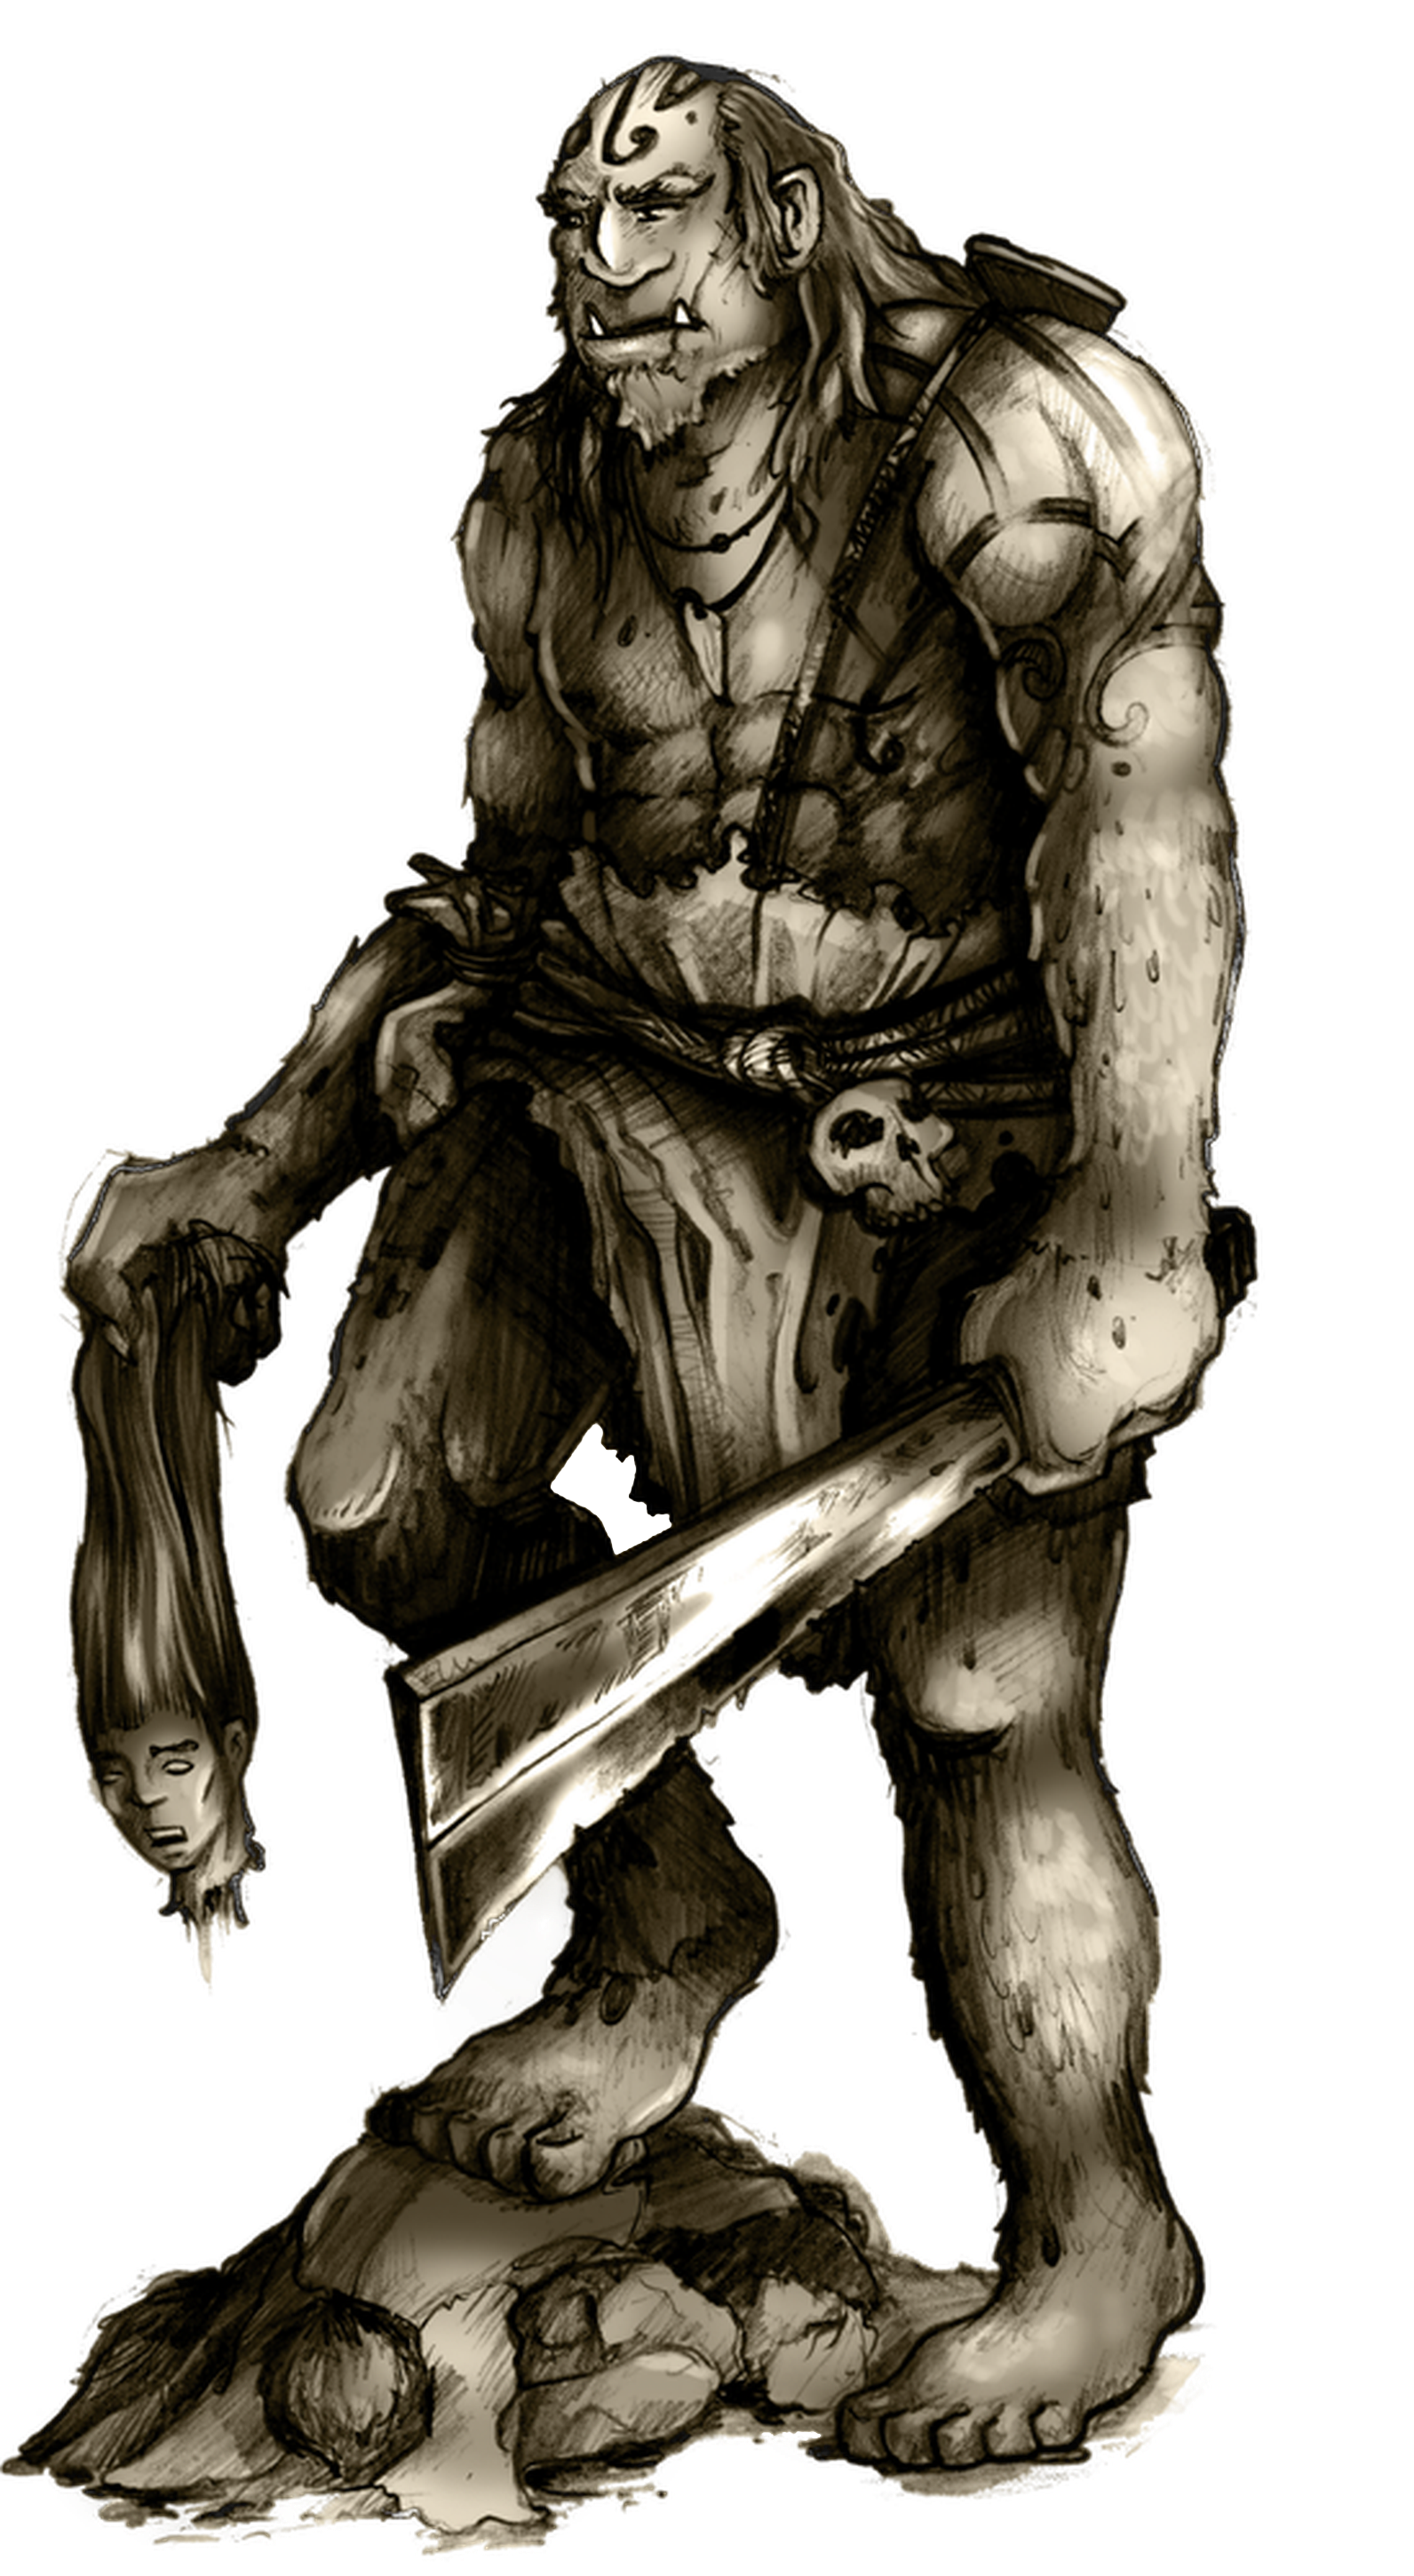
\includegraphics[width=0.33\linewidth]{oger}
\end{center}